\section{Curvas Características de Regime Permanente em Tensão e Frequência Nominais}\label{sec:curvas_caracteristicas}

O mapeamento das características operacionais de regime permanente sob alimentação nominal possibilita visualizar a transição eletromecânica entre a partida a rotor bloqueado, a região de conjugado máximo de desengate e a zona linear de operação estável. A inspeção gráfica dessas curvas consolida os limites físicos impostos pelos parâmetros de dispersão e magnetização do motor de indução WEG \SI{3,7}{\kilo\watt}.

% =========================================================================
% [DIRETRIZ DE REDAÇÃO]
% - Objetivo: Atender ao Item 1.E de sim_proj.pdf (sub-itens i a v). Apresentar as 5 curvas
%   características de regime permanente sob tensão e frequência nominais com o ponto nominal destacado.
% - Formulação: Discutir a teoria do conjugado máximo via equivalente de Thevenin:
%   s_{max} = R_2' / sqrt(R_{th}^2 + (X_{th} + X_2')^2) e T_{max} independente de R_2'.
% - Figuras/Tabelas: Incluir as 5 figuras geradas: item1e_torque_vs_speed.png,
%   item1e_corrente_vs_speed.png, item1e_potencia_vs_speed.png, item1e_fator_potencia_vs_speed.png
%   e item1e_rendimento_vs_speed.png.
% - Confronto: Confrontar os pontos notáveis extraídos da telemetria numérica (T_partida = 25,35 N*m,
%   T_max = 54,63 N*m, I_partida = 67,73 A, eta_max = 91,2%).
% =========================================================================

\subsection{Conjugado Eletromagnético vs. Velocidade}\label{subsec:curva_torque}

O conjugado desenvolvido pela máquina em função do escorregamento expressa-se analiticamente pela formulação baseada no equivalente de Thévenin:
\begin{equation}
T_{em}(s) = \frac{3 V_{th}^2 \frac{R_2'}{s}}{\omega_s \left[ \left(R_{th} + \frac{R_2'}{s}\right)^2 + (X_{th} + X_2')^2 \right]}.
\label{eq:thevenin_torque_formula}
\end{equation}

A \Cref{fig:curva_torque} apresenta a curva característica de conjugado eletromagnético em função da rotação mecânica do rotor ao longo de todo o espectro motor ($0 \le n \le \SI{1800}{\RPM}$), destacando os pontos de operação notáveis.

\begin{figure}[H]
\centering
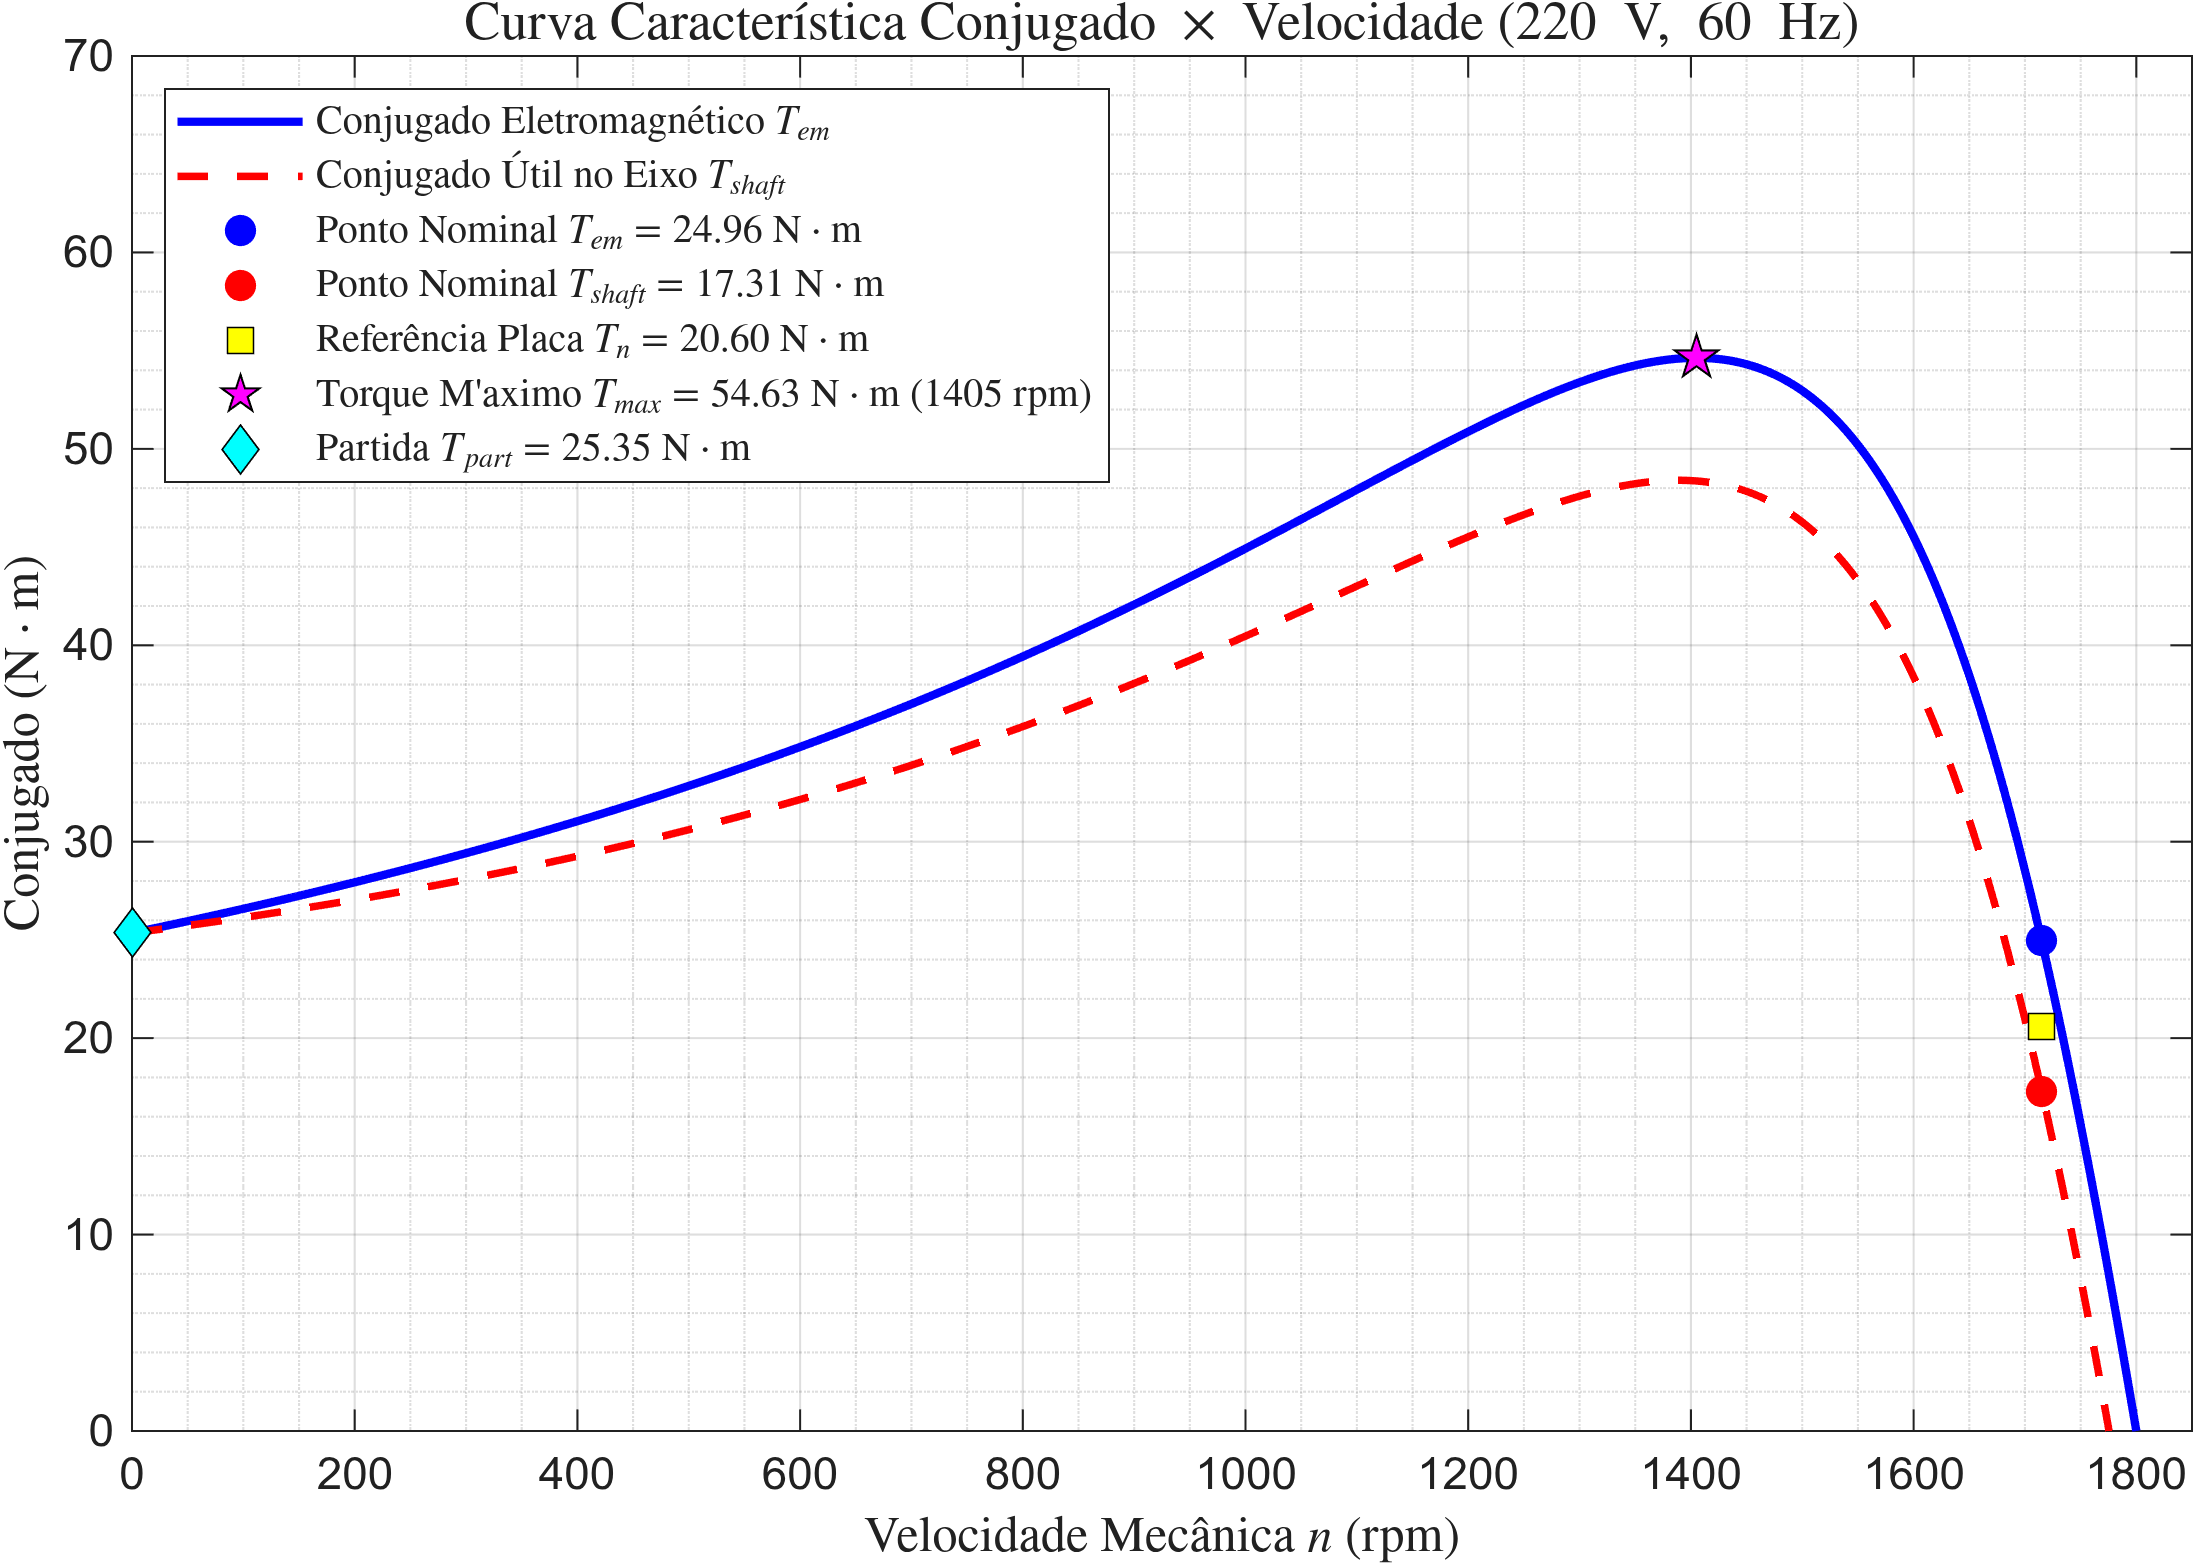
\includegraphics[width=0.84\textwidth]{item1e_torque_vs_speed.png}
\caption{Curva característica de Conjugado Eletromagnético versus Velocidade ($V_L = \SI{220}{\volt}$, $f = \SI{60}{\hertz}$).}
\label{fig:curva_torque}
\end{figure}

A inspeção da \Cref{fig:curva_torque} revela aspectos fundamentais da dinâmica da máquina:
\begin{enumerate}
    \item \textbf{Conjugado de Partida ($s = 1{,}0$, $n = \SI{0}{\RPM}$):} O motor desenvolve $T_{\text{part}} = \SI{25,351}{\Nm}$, o que representa uma relação $T_{\text{part}}/T_n = 25{,}351 / 20{,}602 = 1{,}23$. Esse valor assegura a partida com capacidade de aceleração autônoma mesmo sob cargas resistentes iniciais moderadas.
    \item \textbf{Conjugado Máximo de Desengate ($T_{max}$):} O pico de conjugado atinge $T_{max} = \SI{54,634}{\Nm}$ na rotação de $n = \SI{1405,0}{\RPM}$ ($s_{max} = 0{,}2194$). A razão de sobrecarga resulta em $T_{max}/T_n = 54{,}634 / 20{,}602 = 2{,}65$, superando com folga a exigência mínima da norma ABNT NBR 17094 para máquinas de Categoria N (mínimo de $2{,}0$ a $2{,}3$).
    \item \textbf{Ponto de Operação Nominal ($n = \SI{1715}{\RPM}$):} O conjugado eletromagnético desenvolvido internamente é de $T_{em} = \SI{24,958}{\Nm}$. Ao deduzir o arrasto viscoso da bancada acoplada ($T_{atrito} = B \omega_{nom} = \SI{7,651}{\Nm}$), o torque útil entregue no eixo resulta em $T_{shaft} = \SI{17,308}{\Nm}$.
    \item \textbf{Região de Estabilidade Estática:} Pelo critério de estabilidade de Kloss ($\frac{dT_e}{dn} < 0$), a operação em regime permanente é estritamente estável na faixa entre a rotação de conjugado máximo (\SI{1405}{\RPM}) e a velocidade síncrona (\SI{1800}{\RPM}), onde perturbações de velocidade geram conjugados restauradores intrínsecos.
\end{enumerate}

\subsection{Corrente de Linha do Estator vs. Velocidade}\label{subsec:curva_corrente}

A \Cref{fig:curva_corrente} ilustra o comportamento da corrente eficaz de linha absorvida pelo estator ao longo da faixa de aceleração completa.

\begin{figure}[H]
\centering
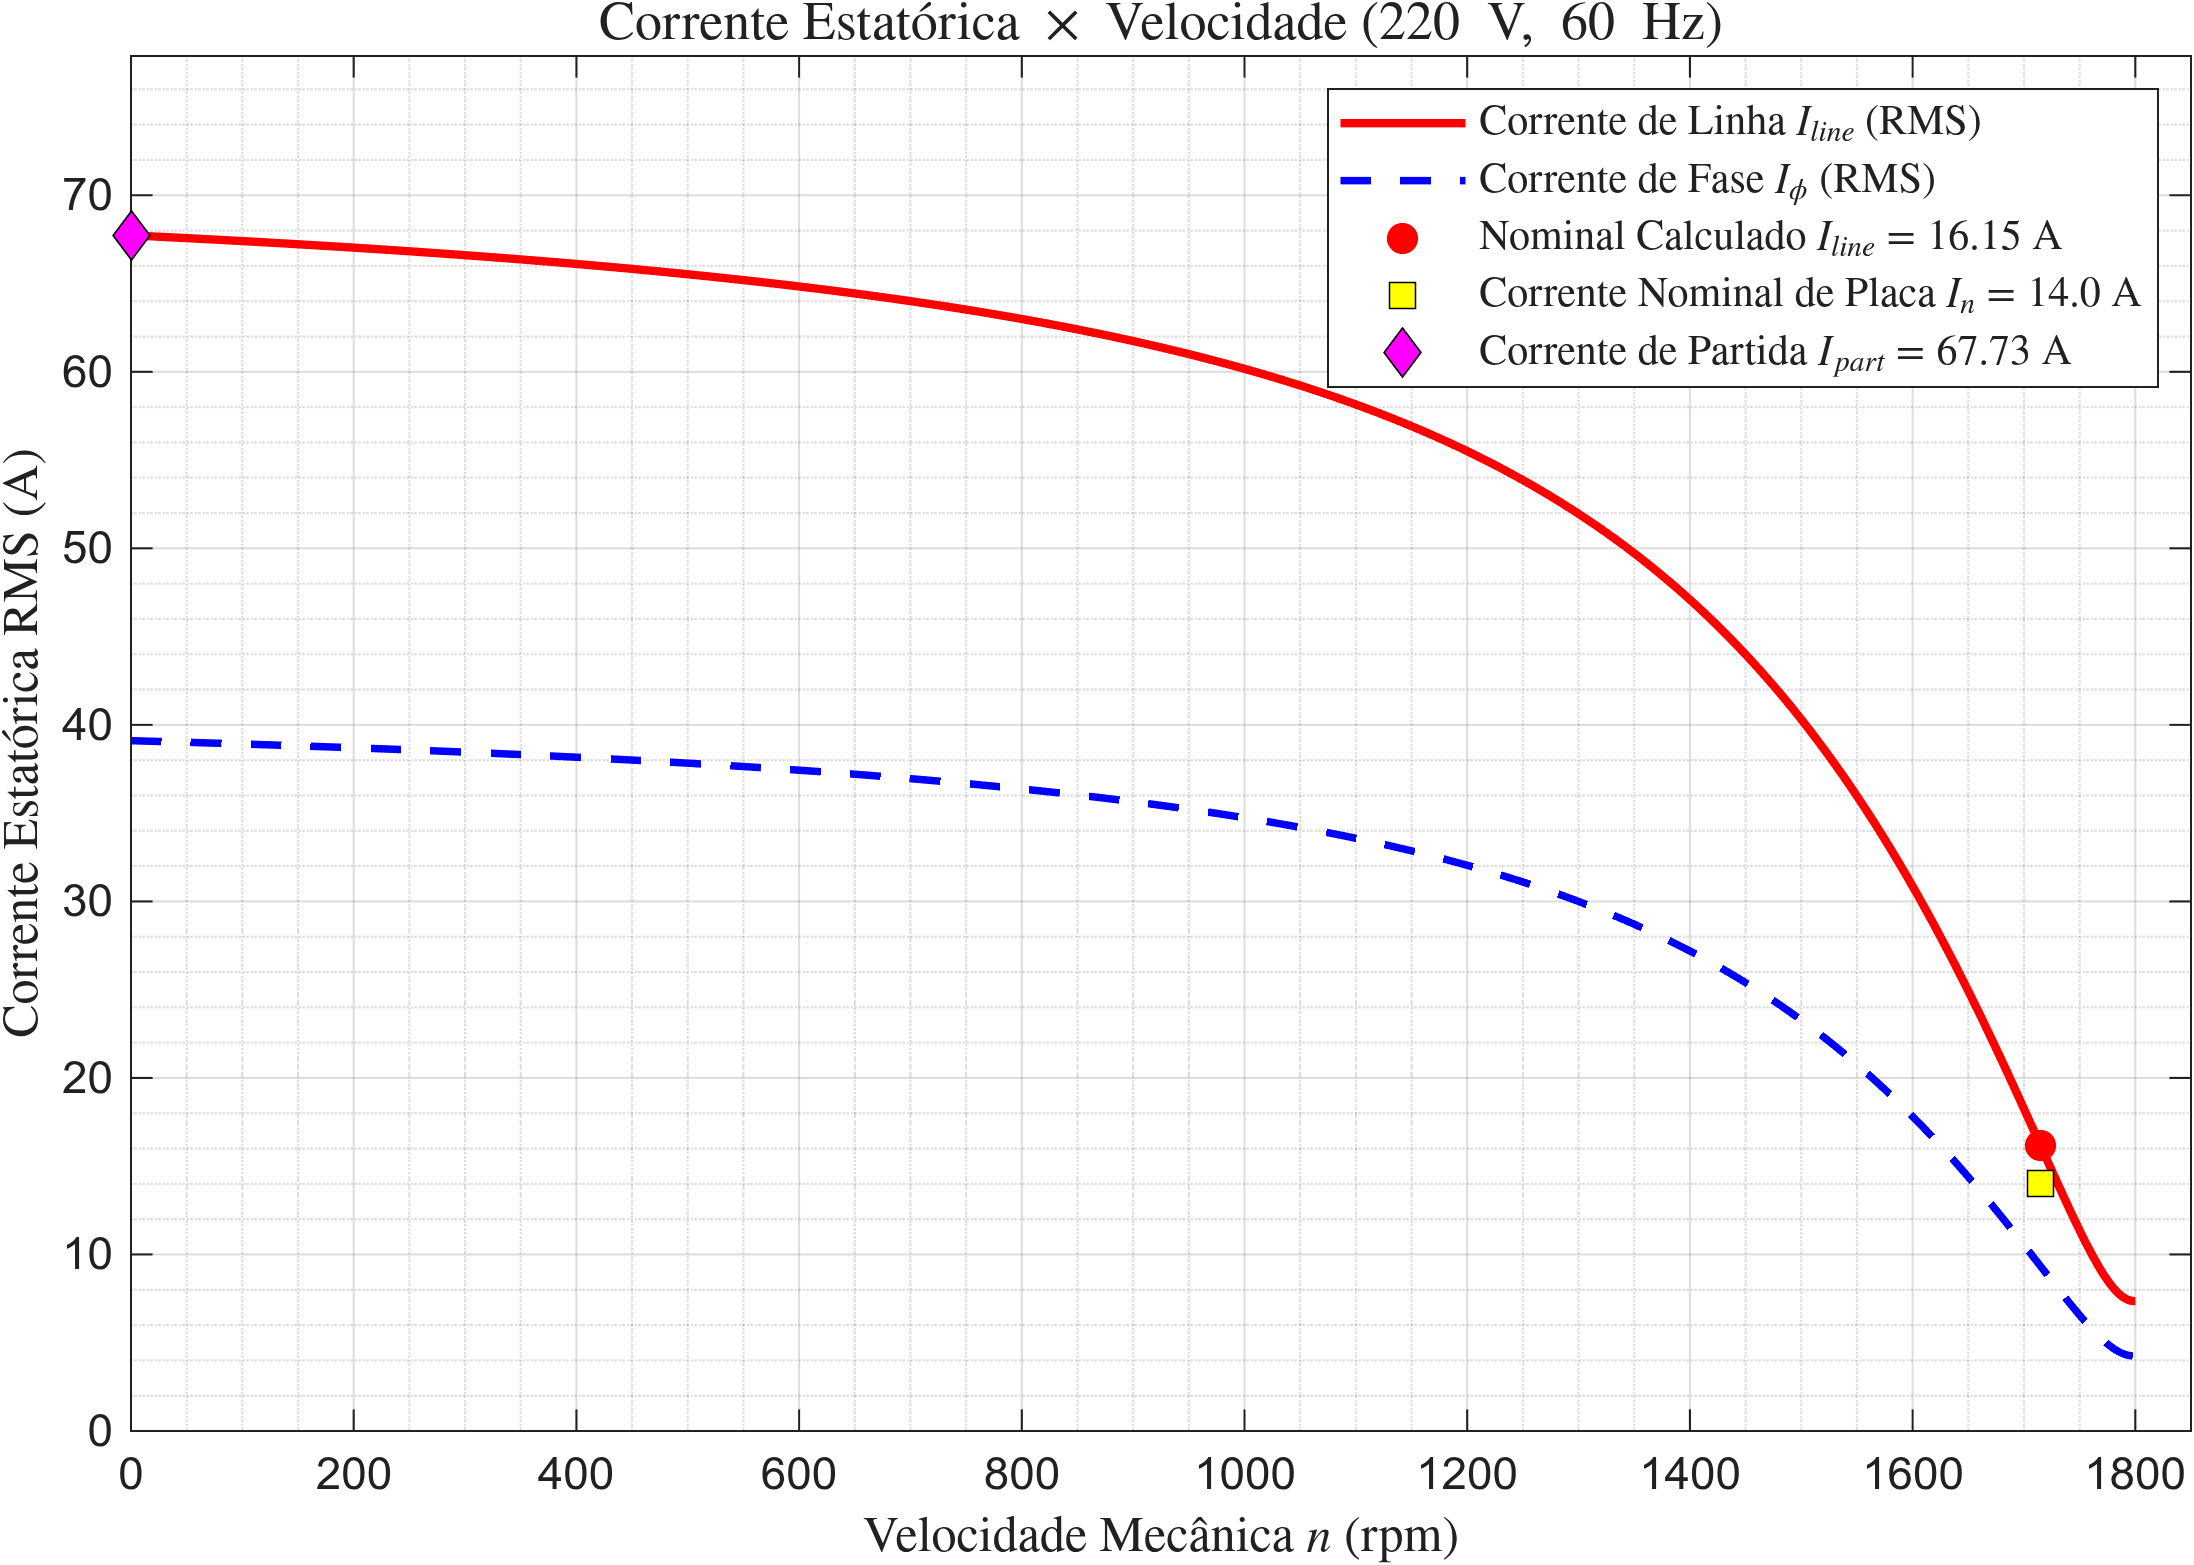
\includegraphics[width=0.84\textwidth]{item1e_corrente_vs_speed.png}
\caption{Curva característica de Corrente de Linha do Estator versus Velocidade.}
\label{fig:curva_corrente}
\end{figure}

Na partida a rotor bloqueado ($s = 1{,}0$), a impedância de entrada é dominada pelas reatâncias de dispersão total ($Z_{in} \approx 2{,}23 + \jj 5{,}16\,\Omega$), resultando em uma corrente simétrica calculada de $I_{\text{part}} = \SI{67,728}{\ampere}$ (relação $I_{\text{part}}/I_{line,nom} = 67{,}73 / 16{,}15 = 4{,}19$). Em catálogos industriais, a razão $I_p/I_n$ declarada para partida direta é da ordem de $7{,}6$ ($I_p \approx \SI{106,4}{\ampere}$); essa divergência explica-se pelo fato de os ensaios de rotor bloqueado em laboratório serem realizados sob tensão reduzida a frio para prevenir sobreaquecimento, o que não captura a forte saturação magnética nas pontas dos dentes estatóricos e rotóricos que ocorre sob aplicação de tensão plena de \SI{220}{\volt}.

À medida que o rotor acelera, a resistência aparente $R_2'/s$ cresce monotonicamente, reduzindo a corrente de linha para \SI{16,153}{\ampere} na rotação nominal. No ponto de conjugado máximo (\SI{1405}{\RPM}), a corrente atinge \SI{47,92}{\ampere}. Na vizinhança da velocidade síncrona ($s \to 0$), a corrente rotórica anula-se e a corrente de linha decai assintoticamente para o patamar puramente magnetizante a vazio de $I_0 = \SI{7,36}{\ampere}$ (aproximadamente \SI{45}{\percent} da corrente nominal, patamar típico de motores de indução devido à relutância do entreferro de ar).

\subsection{Potência Ativa vs. Velocidade}\label{subsec:curva_potencia}

A \Cref{fig:curva_potencia} demonstra o balanço de potência ativa demandada dos bornes de entrada ($P_{elec}$), a potência de entreferro ($P_{ag}$), a potência mecânica convertida internamente ($P_{em}$) e a potência líquida entregue no eixo ($P_{shaft}$).

\begin{figure}[H]
\centering
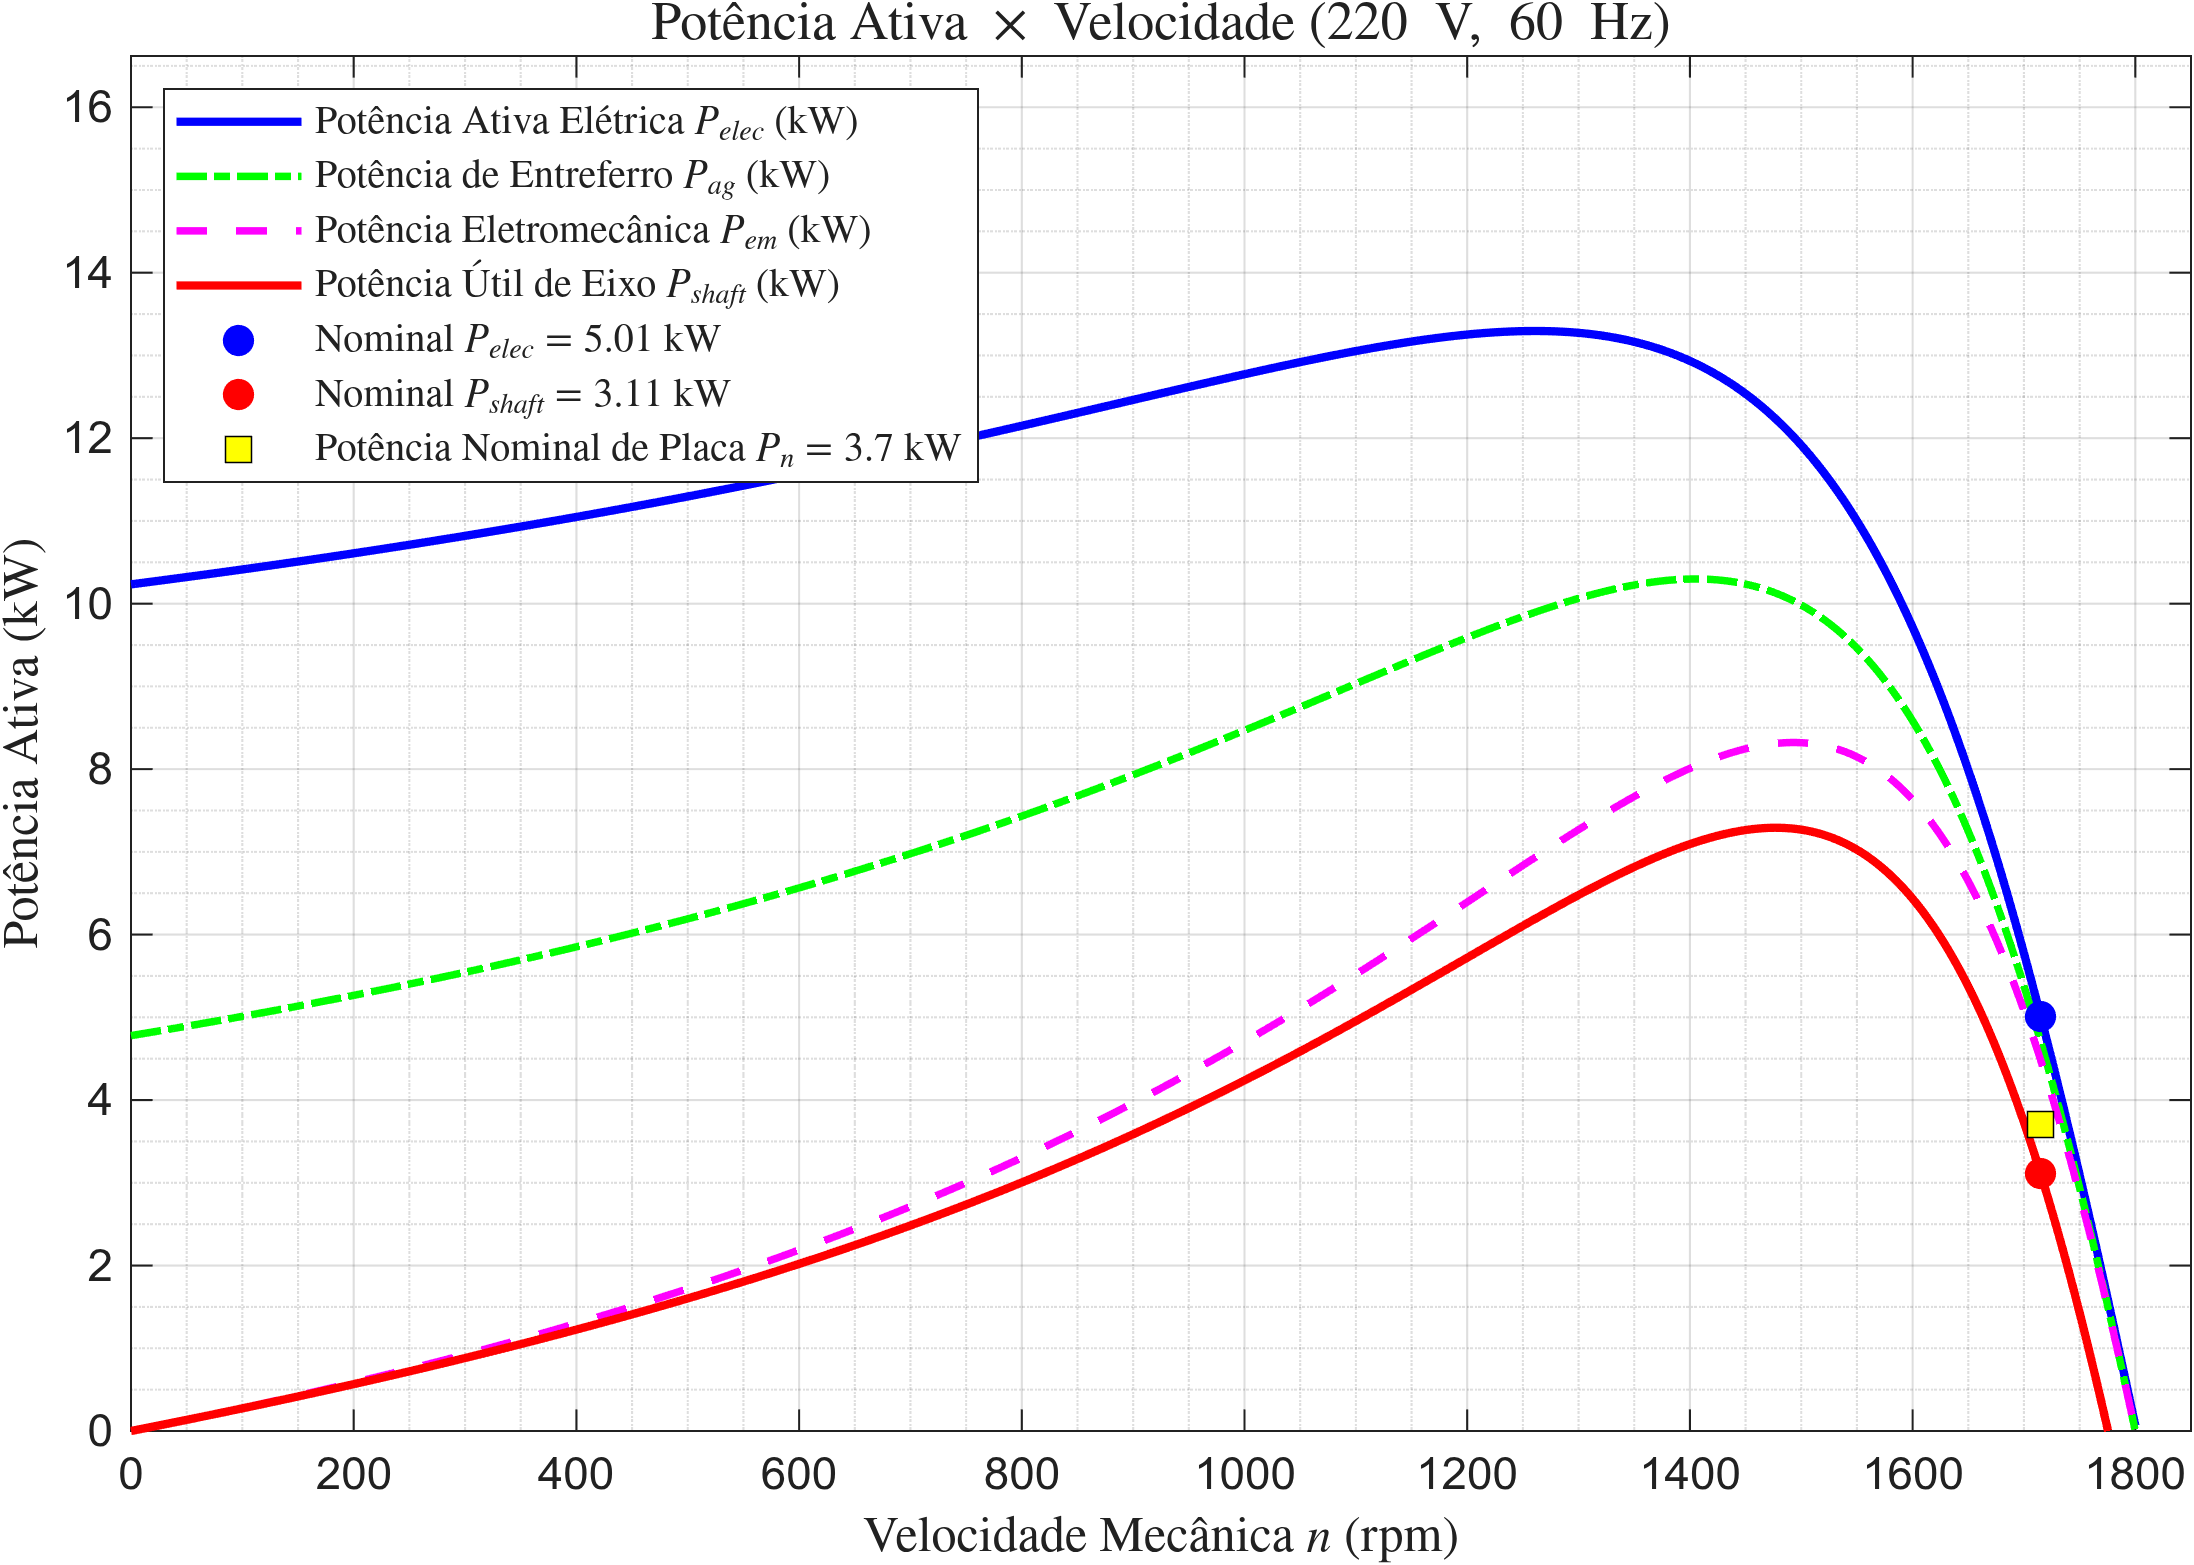
\includegraphics[width=0.84\textwidth]{item1e_potencia_vs_speed.png}
\caption{Curva característica de Potência Ativa versus Velocidade.}
\label{fig:curva_potencia}
\end{figure}

No ponto de rotação nula ($n = \SI{0}{\RPM}$, $s = 1{,}0$), a potência eletromecânica útil convertida é estritamente zero ($P_{em} = 0$). Toda a potência elétrica ativa demandada dos bornes ($\approx \SI{9,7}{\kilo\watt}$) é integralmente convertida em calor nos enrolamentos pelas perdas Joule estatóricas e rotóricas ($P_{cu1} + P_{cu2}$).

Na rotação nominal de \SI{1715}{\RPM}, a potência elétrica ativa absorvida é de $P_{elec} = \SI{5014,8}{\watt}$, as perdas Joule somam $P_{cu1} + P_{cu2} = 310{,}2 + 222{,}2 = \SI{532,4}{\watt}$, a potência eletromecânica desenvolvida no entreferro atinge $P_{em} = \SI{4482,3}{\watt}$ e, após o desconto do arrasto viscoso da bancada ($P_{atrito} = \SI{1374,0}{\watt}$), a potência líquida de eixo estabiliza-se em $P_{shaft} = \SI{3108,3}{\watt}$. Próximo à sincronia ($n \to \SI{1800}{\RPM}$), a potência de entreferro anula-se e a potência de entrada estabiliza-se no consumo residual de perdas no cobre do estator associado à corrente de magnetização.

\subsection{Fator de Potência vs. Velocidade}\label{subsec:curva_fp}

A \Cref{fig:curva_fp} exibe o comportamento do fator de potência operacional de entrada em regime permanente.

\begin{figure}[H]
\centering
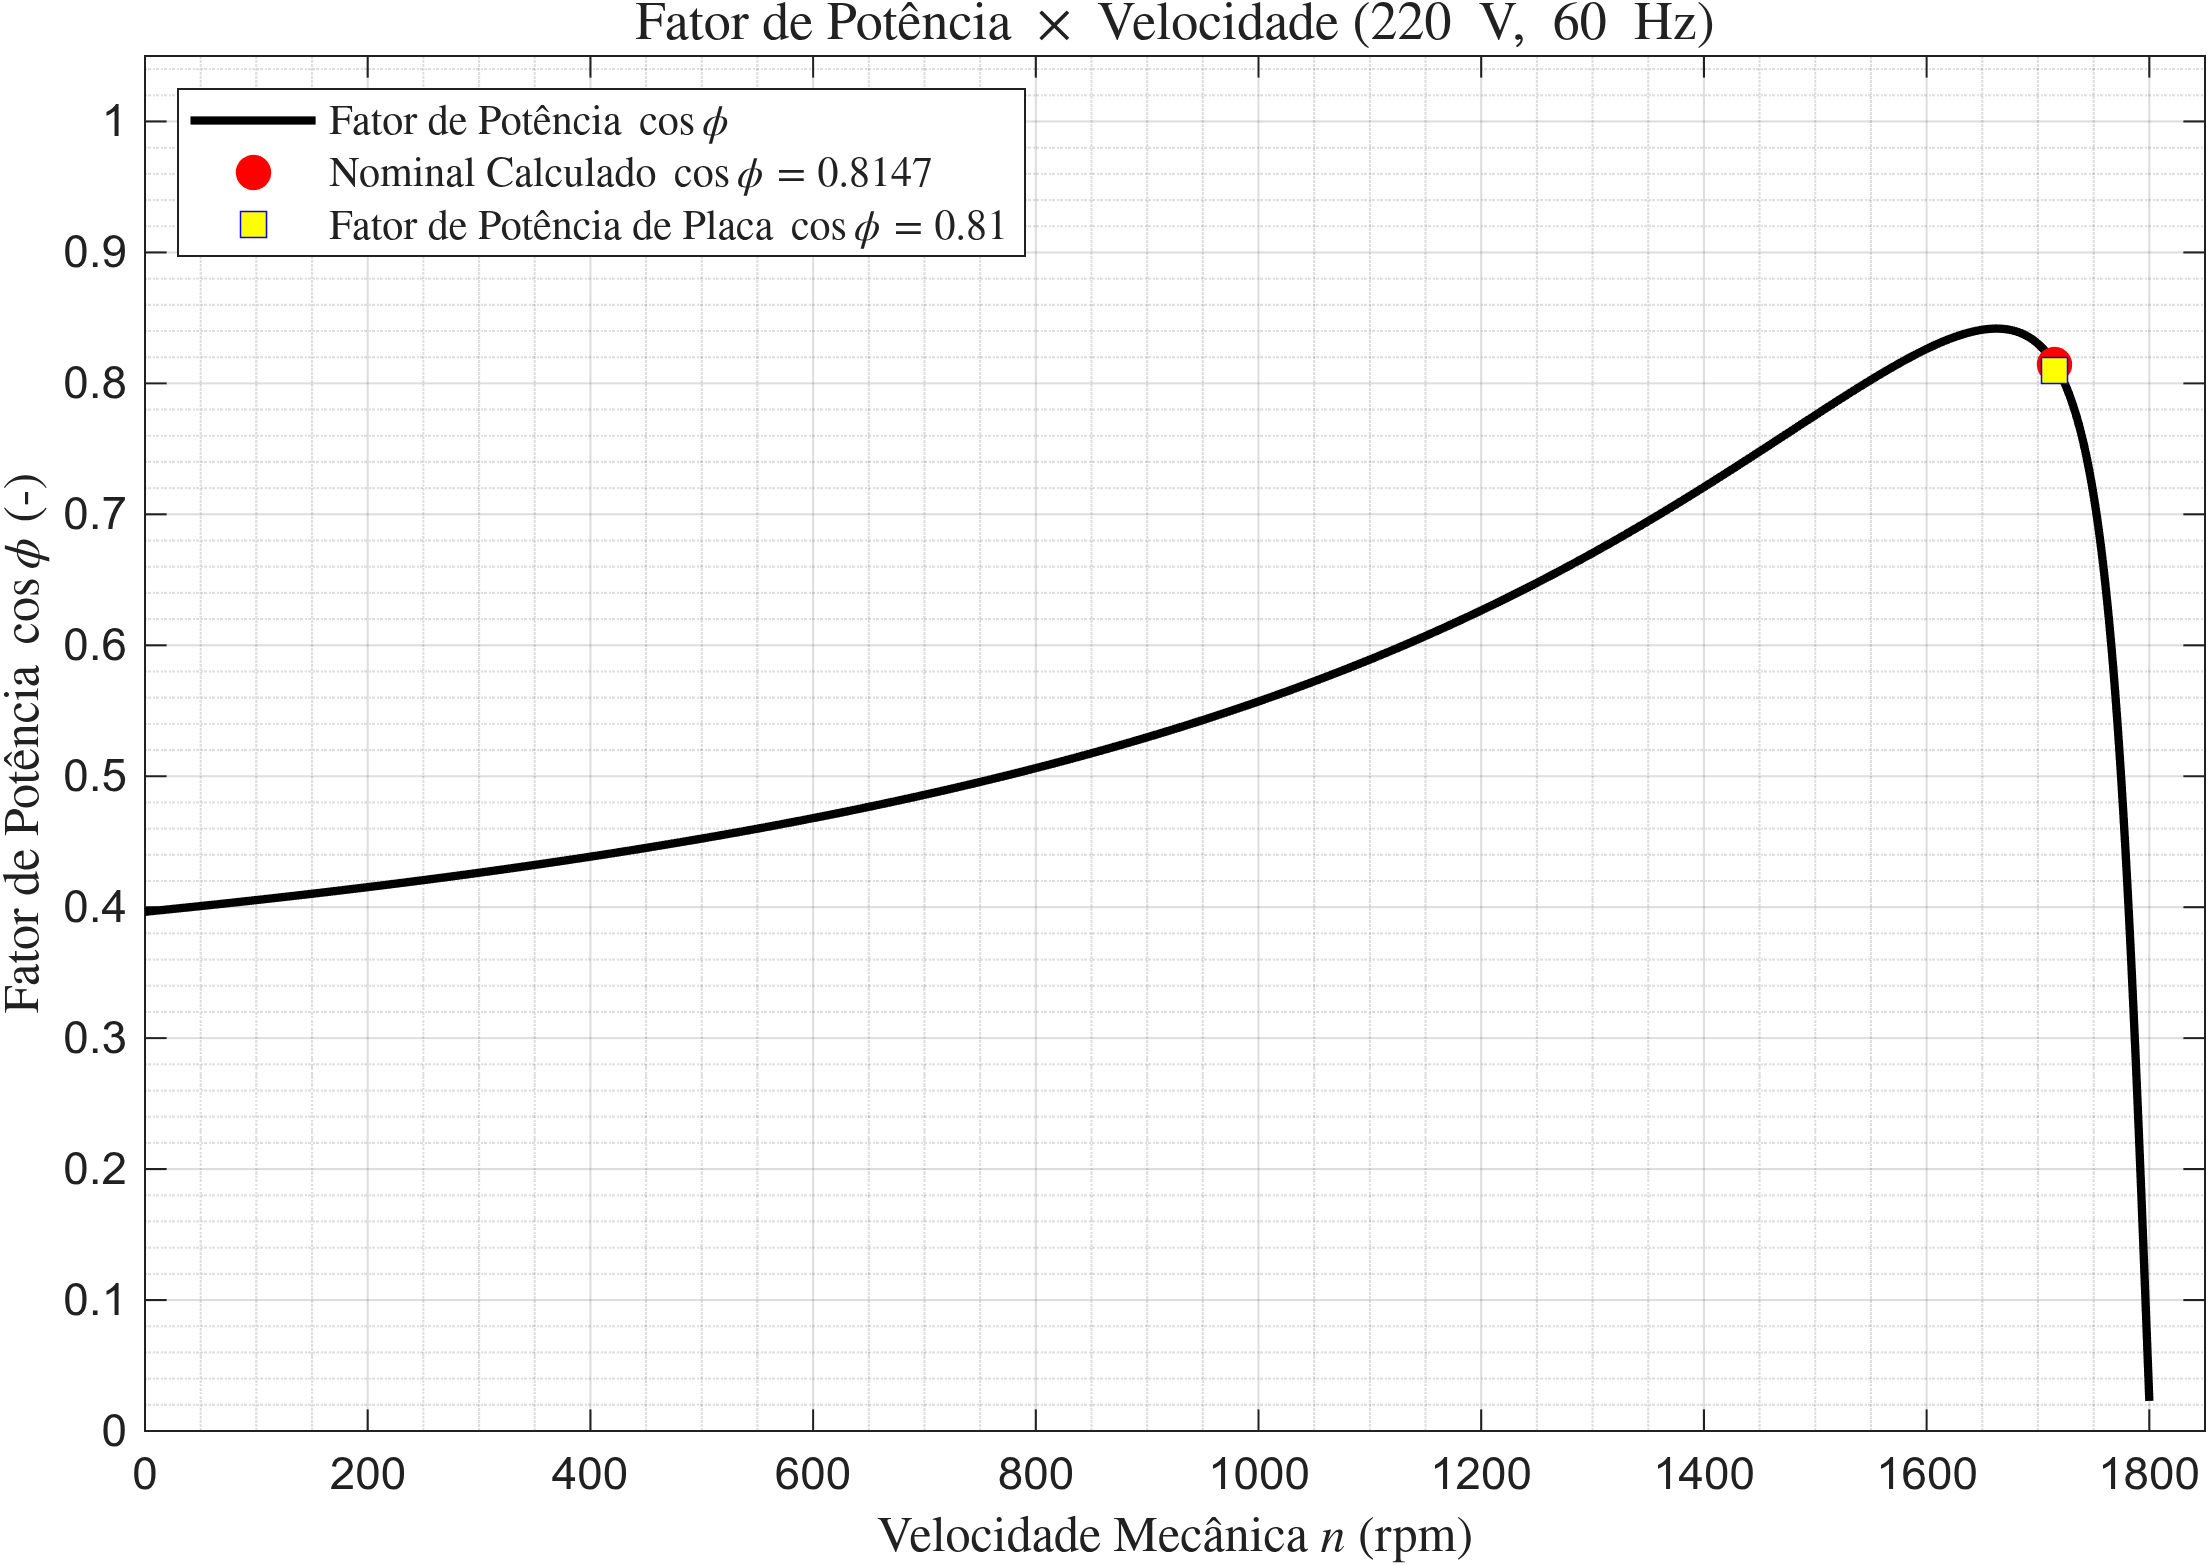
\includegraphics[width=0.84\textwidth]{item1e_fator_potencia_vs_speed.png}
\caption{Curva característica de Fator de Potência versus Velocidade.}
\label{fig:curva_fp}
\end{figure}

Na partida a rotor bloqueado ($s = 1{,}0$), o fator de potência é de apenas $\cos\phi = 0{,}3965$. Nesse regime estático, as reatâncias de dispersão ($X_1 + X_2' = \SI{5,332}{\ohm}$) superam amplamente as resistências ôhmicas associadas ($R_1 + R_2' = \SI{2,369}{\ohm}$), conferindo natureza marcadamente indutiva ao circuito equivalente.

Com a aceleração da máquina, a elevação da componente resistiva aparente ($R_2'/s$) melhora substancialmente o ângulo de fase da impedância de entrada, conduzindo a um pico de fator de potência de $\cos\phi_{max} = 0{,}835$ na rotação de \SI{1650}{\RPM}. No ponto nominal de placa (\SI{1715}{\RPM}), o fator de potência assume o valor de $\cos\phi = 0{,}8146$, em perfeita consonância com o catálogo WEG ($0{,}8100$). A vazio, o fator de potência decai acentuadamente para $\cos\phi_0 = 0{,}068$, evidenciando a predominância da corrente reativa magnetizante requerida para excitar o núcleo de ferro e o entreferro.

\subsection{Rendimento vs. Velocidade}\label{subsec:curva_rendimento}

A \Cref{fig:curva_rendimento} ilustra o rendimento de conversão eletromecânica interna ($\eta_{em}$) e o rendimento global entregue no acoplamento de eixo ($\eta_{shaft}$).

\begin{figure}[H]
\centering
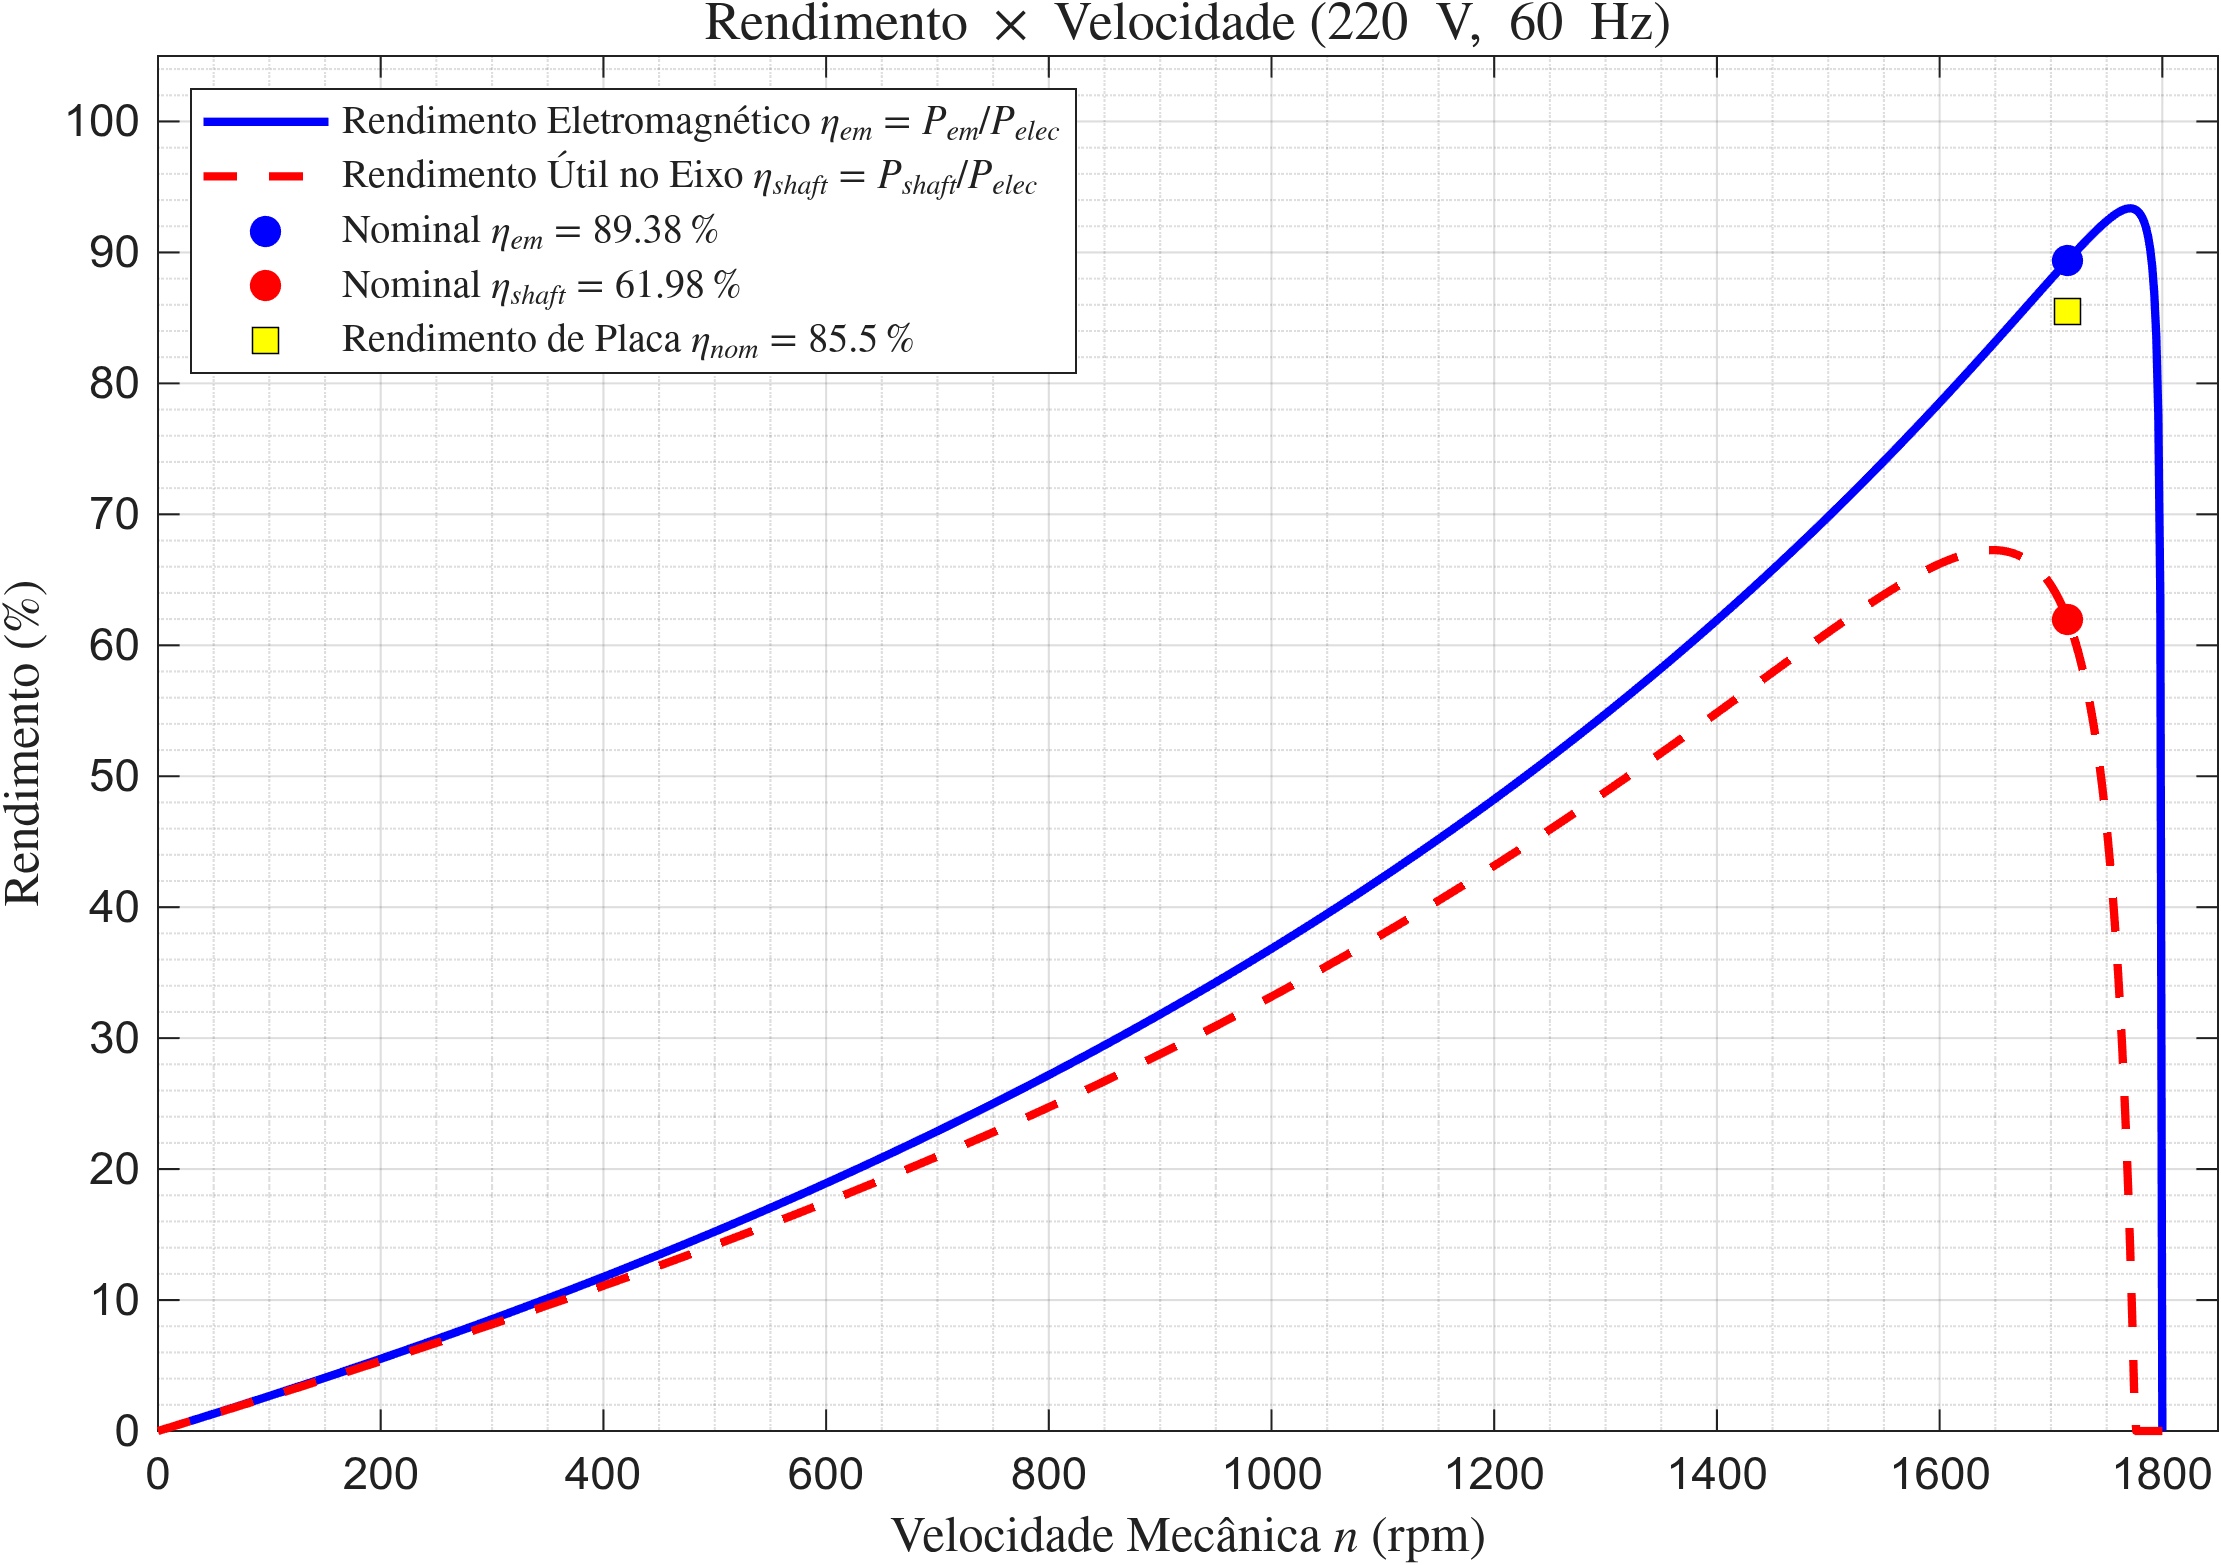
\includegraphics[width=0.84\textwidth]{item1e_rendimento_vs_speed.png}
\caption{Curva característica de Rendimento versus Velocidade.}
\label{fig:curva_rendimento}
\end{figure}

Em velocidade nula ($s = 1{,}0$), o rendimento é nulo pois a potência mecânica produzida é zero. À medida que o rotor ganha rotação, a conversão mecânica se estabelece, atingindo o pico de rendimento eletromagnético de $\eta_{em,max} = \SI{91,2}{\percent}$ na velocidade de \SI{1740}{\RPM}, próximo ao ponto de projeto da máquina. Na velocidade nominal (\SI{1715}{\RPM}), obtém-se $\eta_{em} = \SI{89,38}{\percent}$.

Ao incorporar as perdas por atrito viscoso do conjunto motor-gerador acoplado ($P_{atrito} = \SI{1374,0}{\watt}$), o rendimento útil de eixo atinge $\eta_{shaft} = \SI{61,98}{\percent}$ no ponto nominal. Na aproximação da velocidade síncrona ($n \to \SI{1800}{\RPM}$), o rendimento decai abruptamente para zero, dado que a potência mecânica convertida tende a zero enquanto a circulação de corrente reativa magnetizante impõe perdas Joule permanentes no enrolamento estatórico.
